% !TEX root = presentation.tex
\section{Empirical Evaluation}
\subsection{Experiments}
\frame{\frametitle{Experiments}
  \begin{enumerate}
    \item \textbf{Mutation Score Distribution}
    \item \textbf{Cross-Validation}
    \item \textbf{Prediction on Unknown Data}
    \item Optimization and Generalization
    \item Impact of Amount of Training Data on Prediction Accuracy
  \end{enumerate}
}

\subsubsection{Test Subjects}
\frame{\frametitle{Test Subjects}
  \scriptsize
  \begin{table}
    \centering
    \rowcolors{2}{gray!30}{gray!20}
    \begin{tabular}{|l|>{\raggedleft\arraybackslash}p{0.8cm}|>{\raggedleft\arraybackslash}p{1.2cm}|>{\raggedleft\arraybackslash}p{0.8cm}|>{\raggedleft\arraybackslash}p{1.2cm}|>{\raggedleft\arraybackslash}p{0.8cm}|}
      \hline
      \rowcolor[RGB]{150,160,240}
      \textbf{Test Subject} & \textbf{Source LOC\footnotemark} & \textbf{Source Methods} & \textbf{Test LOC} & \textbf{Test Methods} & \textbf{Test Cases} \\
      \hline \textit{logback-core} & 12118 & 1270 & 8377 & 688 & 286 \\
      \hline \textit{barbecue} & 4790 & 299 & 2910 & 416 & 225 \\
      \hline \textit{jgap } & 28975 & 3017 & 19694 & 1633 & 1355 \\
      \hline \textit{commons-lang} & 19499 & 1196 & 33332 & 2408 & 2050 \\
      \hline \textit{joda-time} & 27139 & 3635 & 51388 & 4755 & 3866 \\
      \hline \textit{openfast} & 11646 & 1447 & 5587 & 421 & 322 \\
      \hline \textit{jsoup} & 10949 & 954 & 2883 & 335 & 319 \\
      \hline \textit{joda-primitives} & 11157 & 1868 & 6989 & 746 & 1810 \\
      \hline \textbf{all} & \textbf{126273} & \textbf{13686} & \textbf{131160} & \textbf{11402} & \textbf{10233} \\
      \hline
    \end{tabular}
    \caption{The eight \alert{open source} test subjects used in the empirical evaluation.}
  \end{table}
  \begin{itemize}
  	\item We use \alert{metrics} from the source code and test suite as \alert{attributes} for \alert{predictions}
 	\end{itemize}
  \footnotetext{Lines of Code (LOC)}
}

\subsection{Mutation Score Distribution}
\frame{\frametitle{Mutation Score Distribution}
  \begin{quote}
    \textit{\textbf{Research Question \#1:} What is the \alert{mutation score distribution} of our test subjects?}
  \end{quote}

  \begin{quote}
    \textit{\textbf{Research Question \#2:} Using the distribution of our test subjects' mutation scores can we identify \alert{three categories} of mutation scores to predict?}
  \end{quote}
}

\subsubsection{Mutation Score Distribution}
\frame{\frametitle{Mutation Score Distribution}
  \begin{figure}[!tb]
    \centering
    \begin{tikzpicture}
    \begin{axis}[
        bar width=1,
        ymajorgrids=true,
        xlabel=Mutation Score (\%),
        ylabel=\# of Methods,
        width=\linewidth,
        height=6.0cm]
        \addplot[ybar,fill=black] file {../thesis/plots/all/evaluation_projects_method_distribution.txt};
    \end{axis}
    \end{tikzpicture}
    \vspace{-2mm}
    \caption{Mutation score \alert{distribution of methods} from all eight test subjects that can be \alert{used for training}.}
  \end{figure}
}

\subsubsection{Mutation Score Categories}
\frame{\frametitle{Mutation Score Categories}
  \begin{table}[!tb]
    \scriptsize
    \centering
    \rowcolors{2}{gray!30}{gray!20}
    \begin{tabular}{|l|>{\raggedleft\arraybackslash}p{2cm}|>{\raggedleft\arraybackslash}p{2cm}|>{\raggedleft\arraybackslash}p{2cm}|}
      \hline
      \rowcolor[RGB]{150,160,240}
      \textbf{Category} & \textbf{Mutation Score Range} & \textbf{Method-Level} \\
      \hline LOW & [0\% -- 70\%) & 1104 \\
      \hline MEDIUM & [70\% -- 90\%) & 1782 \\
      \hline HIGH & [90\% -- 100\%] & 2624 \\
      \hline
    \end{tabular}
    \vspace{-2mm}
    \caption{The available \alert{number of source code units} that fall within the \alert{determined ranges} of mutation scores.}
  \end{table}
}

\subsubsection{Undersampling Categories}
\frame{\frametitle{Undersampling Categories}
  \begin{figure}
    \centering
    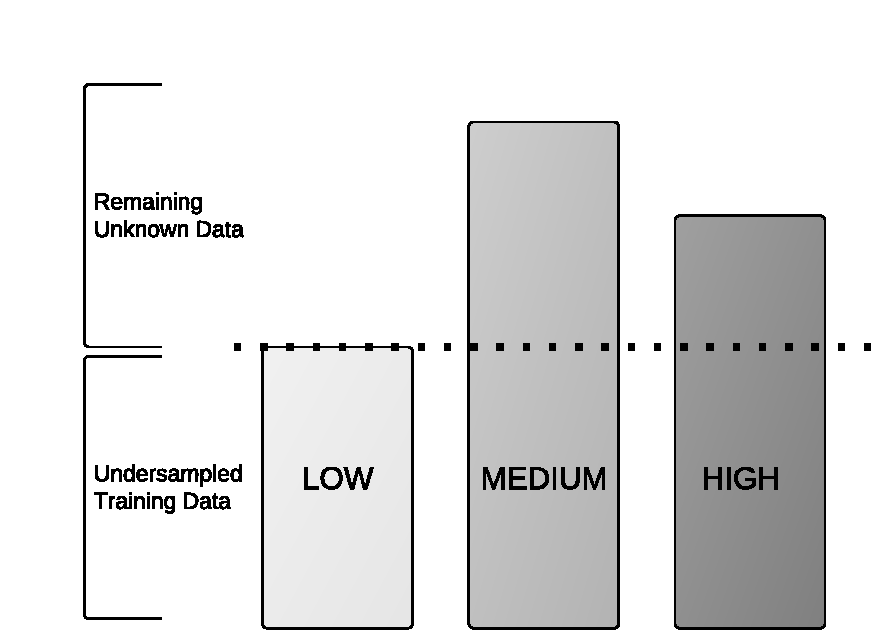
\includegraphics[width=9cm]{../thesis/figures/undersampling.pdf}
    \caption{\alert{Undersampling} a data set for \alert{balanced} categories.}
  \end{figure}
}
  
\subsection{Cross-Validation}
\frame{\frametitle{Cross-Validation}
  \begin{quote}
    \textit{\textbf{Research Question:} Using the test suite and source code data from our test subjects can we identify a \alert{set of features} that \alert{maximize cross-validation accuracy}?}
  \end{quote}
}

\subsection{Feature Sets}
\frame{\frametitle{Feature Sets}
  \begin{itemize}
    \item \alert{\textbf{33} individual metrics} logically grouped into \alert{four feature sets}:
    \begin{itemize}
      \item \ding{172} -- Source Code.
      \item \ding{173} -- Coverage.
      \item \ding{174} -- Accumulated Source Code.
      \item \ding{175} -- Accumulated Test Case.
    \end{itemize}
  \end{itemize}
}

\subsubsection{Evaluating Feature Sets}
\frame{\frametitle{Evaluating Feature Sets}
  \begin{figure}[!tb]
    \centering
    \begin{adjustbox}{max size={.95\textwidth}{.95\textheight}}
      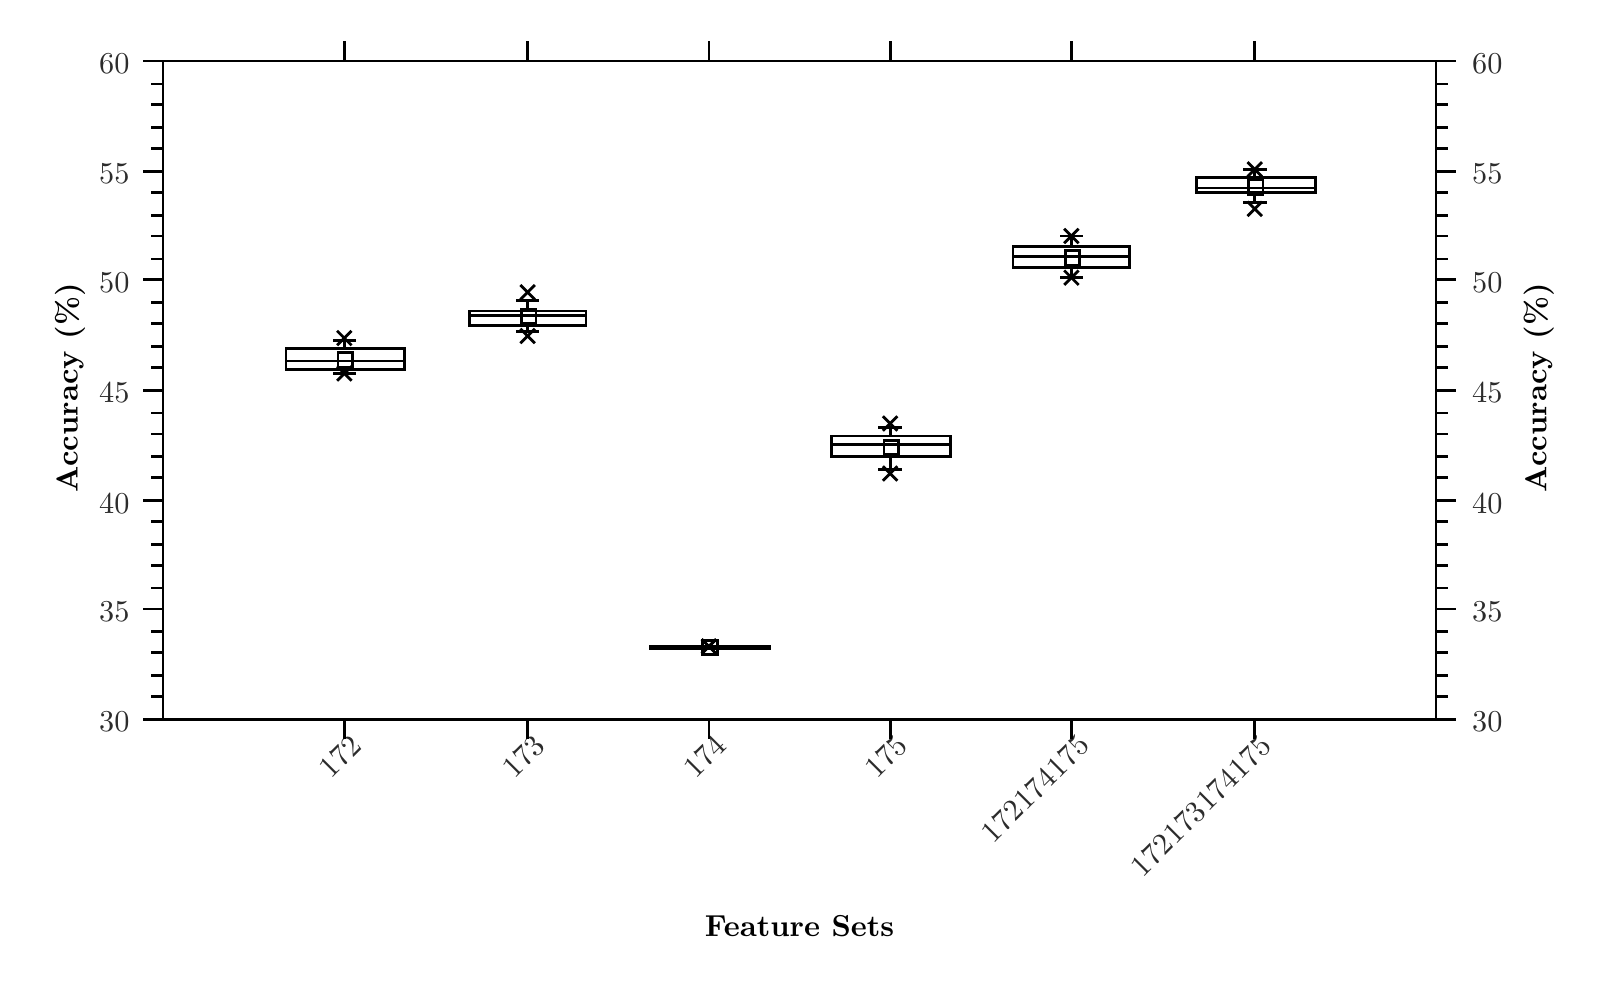
\begin{tikzpicture}{0pt}{0pt}{742pt}{452pt}
	\clip(0pt,452pt) -- (558.587pt,452pt) -- (558.587pt,111.729pt) -- (0pt,111.729pt) -- (0pt,452pt);
\begin{scope}
	\clip(48.9328pt,439.955pt) -- (508.901pt,439.955pt) -- (508.901pt,202.066pt) -- (48.9328pt,202.066pt) -- (48.9328pt,439.955pt);
	\color[rgb]{0,0,0}
	\draw[line width=1pt, line join=miter, line cap=rect](93.3487pt,336.067pt) -- (136.259pt,336.067pt) -- (136.259pt,328.539pt) -- (93.3487pt,328.539pt) -- (93.3487pt,336.067pt);
	\color[rgb]{0,0,0}
	\draw[line width=1pt, line join=miter, line cap=rect](110.663pt,327.033pt) -- (118.192pt,327.033pt);
	\draw[line width=1pt, line join=miter, line cap=rect](110.663pt,339.078pt) -- (118.192pt,339.078pt);
	\draw[line width=1pt, line join=miter, line cap=rect](114.427pt,339.078pt) -- (114.427pt,336.067pt);
	\draw[line width=1pt, line join=miter, line cap=rect](114.427pt,327.033pt) -- (114.427pt,328.539pt);
	\draw[line width=1pt, line join=miter, line cap=rect](93.3487pt,331.55pt) -- (135.506pt,331.55pt);
	\draw[line width=1pt, line join=miter, line cap=rect](112.169pt,329.292pt) -- (116.686pt,324.775pt);
	\draw[line width=1pt, line join=miter, line cap=rect](112.169pt,324.775pt) -- (116.686pt,329.292pt);
	\draw[line width=1pt, line join=miter, line cap=rect](112.169pt,342.089pt) -- (116.686pt,337.572pt);
	\draw[line width=1pt, line join=miter, line cap=rect](112.169pt,337.572pt) -- (116.686pt,342.089pt);
	\draw[line width=1pt, line join=miter, line cap=rect](112.169pt,334.561pt) -- (117.439pt,334.561pt) -- (117.439pt,329.292pt) -- (112.169pt,329.292pt) -- (112.169pt,334.561pt);
	\draw[line width=1pt, line join=miter, line cap=rect](159.596pt,349.618pt) -- (201.754pt,349.618pt) -- (201.754pt,344.348pt) -- (159.596pt,344.348pt) -- (159.596pt,349.618pt);
	\draw[line width=1pt, line join=miter, line cap=rect](176.911pt,342.089pt) -- (184.439pt,342.089pt);
	\draw[line width=1pt, line join=miter, line cap=rect](176.911pt,353.382pt) -- (184.439pt,353.382pt);
	\draw[line width=1pt, line join=miter, line cap=rect](180.675pt,353.382pt) -- (180.675pt,349.618pt);
	\draw[line width=1pt, line join=miter, line cap=rect](180.675pt,342.089pt) -- (180.675pt,344.348pt);
	\draw[line width=1pt, line join=miter, line cap=rect](159.596pt,348.112pt) -- (201.754pt,348.112pt);
	\draw[line width=1pt, line join=miter, line cap=rect](178.417pt,342.842pt) -- (182.933pt,338.325pt);
	\draw[line width=1pt, line join=miter, line cap=rect](178.417pt,338.325pt) -- (182.933pt,342.842pt);
	\draw[line width=1pt, line join=miter, line cap=rect](178.417pt,358.651pt) -- (182.933pt,354.134pt);
	\draw[line width=1pt, line join=miter, line cap=rect](178.417pt,354.134pt) -- (182.933pt,358.651pt);
	\draw[line width=1pt, line join=miter, line cap=rect](178.417pt,350.37pt) -- (183.686pt,350.37pt) -- (183.686pt,345.101pt) -- (178.417pt,345.101pt) -- (178.417pt,350.37pt);
	\draw[line width=1pt, line join=miter, line cap=rect](225.091pt,228.415pt) -- (268.001pt,228.415pt) -- (268.001pt,227.662pt) -- (225.091pt,227.662pt) -- (225.091pt,228.415pt);
	\draw[line width=1pt, line join=miter, line cap=rect](242.406pt,228.415pt) -- (249.934pt,228.415pt);
	\draw[line width=1pt, line join=miter, line cap=rect](242.406pt,228.415pt) -- (249.934pt,228.415pt);
	\draw[line width=1pt, line join=miter, line cap=rect](225.091pt,228.415pt) -- (267.248pt,228.415pt);
	\draw[line width=1pt, line join=miter, line cap=rect](243.911pt,230.673pt) -- (248.428pt,226.156pt);
	\draw[line width=1pt, line join=miter, line cap=rect](243.911pt,226.156pt) -- (248.428pt,230.673pt);
	\draw[line width=1pt, line join=miter, line cap=rect](243.911pt,230.673pt) -- (248.428pt,226.156pt);
	\draw[line width=1pt, line join=miter, line cap=rect](243.911pt,226.156pt) -- (248.428pt,230.673pt);
	\draw[line width=1pt, line join=miter, line cap=rect](243.911pt,230.673pt) -- (249.181pt,230.673pt) -- (249.181pt,225.403pt) -- (243.911pt,225.403pt) -- (243.911pt,230.673pt);
	\draw[line width=1pt, line join=miter, line cap=rect](290.586pt,304.449pt) -- (333.496pt,304.449pt) -- (333.496pt,296.921pt) -- (290.586pt,296.921pt) -- (290.586pt,304.449pt);
	\draw[line width=1pt, line join=miter, line cap=rect](307.9pt,292.404pt) -- (315.428pt,292.404pt);
	\draw[line width=1pt, line join=miter, line cap=rect](307.9pt,307.46pt) -- (315.428pt,307.46pt);
	\draw[line width=1pt, line join=miter, line cap=rect](311.664pt,307.46pt) -- (311.664pt,304.449pt);
	\draw[line width=1pt, line join=miter, line cap=rect](311.664pt,292.404pt) -- (311.664pt,296.921pt);
	\draw[line width=1pt, line join=miter, line cap=rect](290.586pt,301.438pt) -- (332.743pt,301.438pt);
	\draw[line width=1pt, line join=miter, line cap=rect](309.406pt,293.157pt) -- (313.923pt,288.64pt);
	\draw[line width=1pt, line join=miter, line cap=rect](309.406pt,288.64pt) -- (313.923pt,293.157pt);
	\draw[line width=1pt, line join=miter, line cap=rect](309.406pt,311.224pt) -- (313.923pt,306.707pt);
	\draw[line width=1pt, line join=miter, line cap=rect](309.406pt,306.707pt) -- (313.923pt,311.224pt);
	\draw[line width=1pt, line join=miter, line cap=rect](309.406pt,302.943pt) -- (314.676pt,302.943pt) -- (314.676pt,297.673pt) -- (309.406pt,297.673pt) -- (309.406pt,302.943pt);
	\draw[line width=1pt, line join=miter, line cap=rect](356.08pt,372.955pt) -- (398.238pt,372.955pt) -- (398.238pt,365.427pt) -- (356.08pt,365.427pt) -- (356.08pt,372.955pt);
	\draw[line width=1pt, line join=miter, line cap=rect](373.395pt,361.663pt) -- (380.923pt,361.663pt);
	\draw[line width=1pt, line join=miter, line cap=rect](373.395pt,376.719pt) -- (380.923pt,376.719pt);
	\draw[line width=1pt, line join=miter, line cap=rect](377.159pt,376.719pt) -- (377.159pt,372.955pt);
	\draw[line width=1pt, line join=miter, line cap=rect](377.159pt,361.663pt) -- (377.159pt,365.427pt);
	\draw[line width=1pt, line join=miter, line cap=rect](356.08pt,369.191pt) -- (398.238pt,369.191pt);
	\draw[line width=1pt, line join=miter, line cap=rect](374.901pt,363.921pt) -- (379.418pt,359.404pt);
	\draw[line width=1pt, line join=miter, line cap=rect](374.901pt,359.404pt) -- (379.418pt,363.921pt);
	\draw[line width=1pt, line join=miter, line cap=rect](374.901pt,378.977pt) -- (379.418pt,374.46pt);
	\draw[line width=1pt, line join=miter, line cap=rect](374.901pt,374.46pt) -- (379.418pt,378.977pt);
	\draw[line width=1pt, line join=miter, line cap=rect](374.901pt,371.449pt) -- (380.17pt,371.449pt) -- (380.17pt,366.179pt) -- (374.901pt,366.179pt) -- (374.901pt,371.449pt);
	\draw[line width=1pt, line join=miter, line cap=rect](422.328pt,397.798pt) -- (465.238pt,397.798pt) -- (465.238pt,392.528pt) -- (422.328pt,392.528pt) -- (422.328pt,397.798pt);
	\draw[line width=1pt, line join=miter, line cap=rect](439.642pt,388.764pt) -- (447.171pt,388.764pt);
	\draw[line width=1pt, line join=miter, line cap=rect](439.642pt,400.809pt) -- (447.171pt,400.809pt);
	\draw[line width=1pt, line join=miter, line cap=rect](443.407pt,400.809pt) -- (443.407pt,397.798pt);
	\draw[line width=1pt, line join=miter, line cap=rect](443.407pt,388.764pt) -- (443.407pt,392.528pt);
	\draw[line width=1pt, line join=miter, line cap=rect](422.328pt,394.033pt) -- (464.485pt,394.033pt);
	\draw[line width=1pt, line join=miter, line cap=rect](441.148pt,388.764pt) -- (445.665pt,384.247pt);
	\draw[line width=1pt, line join=miter, line cap=rect](441.148pt,384.247pt) -- (445.665pt,388.764pt);
	\draw[line width=1pt, line join=miter, line cap=rect](441.148pt,403.067pt) -- (445.665pt,398.55pt);
	\draw[line width=1pt, line join=miter, line cap=rect](441.148pt,398.55pt) -- (445.665pt,403.067pt);
	\draw[line width=1pt, line join=miter, line cap=rect](441.148pt,397.045pt) -- (446.418pt,397.045pt) -- (446.418pt,391.775pt) -- (441.148pt,391.775pt) -- (441.148pt,397.045pt);
\end{scope}
\begin{scope}
	\color[rgb]{0,0,0}
	\pgftext[center, base, at={\pgfpoint{18.0675pt}{321.763pt}},rotate=90]{\fontsize{11}{0}\selectfont{\textbf{Accuracy (\%)}}}
	\color[rgb]{0.172549,0.172549,0.172549}
	\pgftext[center, base, at={\pgfpoint{31.3358pt}{197.549pt}}]{\fontsize{11}{0}\selectfont{30}}
	\pgftext[center, base, at={\pgfpoint{31.3358pt}{237.448pt}}]{\fontsize{11}{0}\selectfont{35}}
	\pgftext[center, base, at={\pgfpoint{31.3358pt}{276.595pt}}]{\fontsize{11}{0}\selectfont{40}}
	\pgftext[center, base, at={\pgfpoint{31.3358pt}{316.494pt}}]{\fontsize{11}{0}\selectfont{45}}
	\pgftext[center, base, at={\pgfpoint{31.3358pt}{356.393pt}}]{\fontsize{11}{0}\selectfont{50}}
	\pgftext[center, base, at={\pgfpoint{31.3358pt}{395.539pt}}]{\fontsize{11}{0}\selectfont{55}}
	\pgftext[center, base, at={\pgfpoint{31.3358pt}{435.438pt}}]{\fontsize{11}{0}\selectfont{60}}
	\color[rgb]{0,0,0}
	\draw[line width=1pt, line join=bevel, line cap=rect](48.9328pt,210.347pt) -- (45.1688pt,210.347pt);
	\draw[line width=1pt, line join=bevel, line cap=rect](48.9328pt,217.875pt) -- (45.1688pt,217.875pt);
	\draw[line width=1pt, line join=bevel, line cap=rect](48.9328pt,226.156pt) -- (45.1688pt,226.156pt);
	\draw[line width=1pt, line join=bevel, line cap=rect](48.9328pt,233.684pt) -- (45.1688pt,233.684pt);
	\draw[line width=1pt, line join=bevel, line cap=rect](48.9328pt,249.493pt) -- (45.1688pt,249.493pt);
	\draw[line width=1pt, line join=bevel, line cap=rect](48.9328pt,257.774pt) -- (45.1688pt,257.774pt);
	\draw[line width=1pt, line join=bevel, line cap=rect](48.9328pt,265.303pt) -- (45.1688pt,265.303pt);
	\draw[line width=1pt, line join=bevel, line cap=rect](48.9328pt,273.583pt) -- (45.1688pt,273.583pt);
	\draw[line width=1pt, line join=bevel, line cap=rect](48.9328pt,289.393pt) -- (45.1688pt,289.393pt);
	\draw[line width=1pt, line join=bevel, line cap=rect](48.9328pt,296.921pt) -- (45.1688pt,296.921pt);
	\draw[line width=1pt, line join=bevel, line cap=rect](48.9328pt,305.202pt) -- (45.1688pt,305.202pt);
	\draw[line width=1pt, line join=bevel, line cap=rect](48.9328pt,312.73pt) -- (45.1688pt,312.73pt);
	\draw[line width=1pt, line join=bevel, line cap=rect](48.9328pt,329.292pt) -- (45.1688pt,329.292pt);
	\draw[line width=1pt, line join=bevel, line cap=rect](48.9328pt,336.82pt) -- (45.1688pt,336.82pt);
	\draw[line width=1pt, line join=bevel, line cap=rect](48.9328pt,345.101pt) -- (45.1688pt,345.101pt);
	\draw[line width=1pt, line join=bevel, line cap=rect](48.9328pt,352.629pt) -- (45.1688pt,352.629pt);
	\draw[line width=1pt, line join=bevel, line cap=rect](48.9328pt,368.438pt) -- (45.1688pt,368.438pt);
	\draw[line width=1pt, line join=bevel, line cap=rect](48.9328pt,376.719pt) -- (45.1688pt,376.719pt);
	\draw[line width=1pt, line join=bevel, line cap=rect](48.9328pt,384.247pt) -- (45.1688pt,384.247pt);
	\draw[line width=1pt, line join=bevel, line cap=rect](48.9328pt,392.528pt) -- (45.1688pt,392.528pt);
	\draw[line width=1pt, line join=bevel, line cap=rect](48.9328pt,408.337pt) -- (45.1688pt,408.337pt);
	\draw[line width=1pt, line join=bevel, line cap=rect](48.9328pt,415.865pt) -- (45.1688pt,415.865pt);
	\draw[line width=1pt, line join=bevel, line cap=rect](48.9328pt,424.146pt) -- (45.1688pt,424.146pt);
	\draw[line width=1pt, line join=bevel, line cap=rect](48.9328pt,431.674pt) -- (45.1688pt,431.674pt);
	\draw[line width=1pt, line join=bevel, line cap=rect](48.9328pt,202.066pt) -- (42.1575pt,202.066pt);
	\draw[line width=1pt, line join=bevel, line cap=rect](48.9328pt,241.965pt) -- (42.1575pt,241.965pt);
	\draw[line width=1pt, line join=bevel, line cap=rect](48.9328pt,281.112pt) -- (42.1575pt,281.112pt);
	\draw[line width=1pt, line join=bevel, line cap=rect](48.9328pt,321.011pt) -- (42.1575pt,321.011pt);
	\draw[line width=1pt, line join=bevel, line cap=rect](48.9328pt,360.91pt) -- (42.1575pt,360.91pt);
	\draw[line width=1pt, line join=bevel, line cap=rect](48.9328pt,400.056pt) -- (42.1575pt,400.056pt);
	\draw[line width=1pt, line join=bevel, line cap=rect](48.9328pt,439.955pt) -- (42.1575pt,439.955pt);
	\draw[line width=1pt, line join=bevel, line cap=rect](48.9328pt,439.955pt) -- (48.9328pt,202.066pt);
	\pgftext[center, base, at={\pgfpoint{548.8pt}{321.763pt}},rotate=90]{\fontsize{11}{0}\selectfont{\textbf{Accuracy (\%)}}}
	\color[rgb]{0.172549,0.172549,0.172549}
	\pgftext[center, base, at={\pgfpoint{527.439pt}{197.549pt}}]{\fontsize{11}{0}\selectfont{30}}
	\pgftext[center, base, at={\pgfpoint{527.439pt}{237.448pt}}]{\fontsize{11}{0}\selectfont{35}}
	\pgftext[center, base, at={\pgfpoint{527.439pt}{276.595pt}}]{\fontsize{11}{0}\selectfont{40}}
	\pgftext[center, base, at={\pgfpoint{527.439pt}{316.494pt}}]{\fontsize{11}{0}\selectfont{45}}
	\pgftext[center, base, at={\pgfpoint{527.439pt}{356.393pt}}]{\fontsize{11}{0}\selectfont{50}}
	\pgftext[center, base, at={\pgfpoint{527.439pt}{395.539pt}}]{\fontsize{11}{0}\selectfont{55}}
	\pgftext[center, base, at={\pgfpoint{527.439pt}{435.438pt}}]{\fontsize{11}{0}\selectfont{60}}
	\color[rgb]{0,0,0}
	\draw[line width=1pt, line join=bevel, line cap=rect](508.901pt,210.347pt) -- (512.665pt,210.347pt);
	\draw[line width=1pt, line join=bevel, line cap=rect](508.901pt,217.875pt) -- (512.665pt,217.875pt);
	\draw[line width=1pt, line join=bevel, line cap=rect](508.901pt,226.156pt) -- (512.665pt,226.156pt);
	\draw[line width=1pt, line join=bevel, line cap=rect](508.901pt,233.684pt) -- (512.665pt,233.684pt);
	\draw[line width=1pt, line join=bevel, line cap=rect](508.901pt,249.493pt) -- (512.665pt,249.493pt);
	\draw[line width=1pt, line join=bevel, line cap=rect](508.901pt,257.774pt) -- (512.665pt,257.774pt);
	\draw[line width=1pt, line join=bevel, line cap=rect](508.901pt,265.303pt) -- (512.665pt,265.303pt);
	\draw[line width=1pt, line join=bevel, line cap=rect](508.901pt,273.583pt) -- (512.665pt,273.583pt);
	\draw[line width=1pt, line join=bevel, line cap=rect](508.901pt,289.393pt) -- (512.665pt,289.393pt);
	\draw[line width=1pt, line join=bevel, line cap=rect](508.901pt,296.921pt) -- (512.665pt,296.921pt);
	\draw[line width=1pt, line join=bevel, line cap=rect](508.901pt,305.202pt) -- (512.665pt,305.202pt);
	\draw[line width=1pt, line join=bevel, line cap=rect](508.901pt,312.73pt) -- (512.665pt,312.73pt);
	\draw[line width=1pt, line join=bevel, line cap=rect](508.901pt,329.292pt) -- (512.665pt,329.292pt);
	\draw[line width=1pt, line join=bevel, line cap=rect](508.901pt,336.82pt) -- (512.665pt,336.82pt);
	\draw[line width=1pt, line join=bevel, line cap=rect](508.901pt,345.101pt) -- (512.665pt,345.101pt);
	\draw[line width=1pt, line join=bevel, line cap=rect](508.901pt,352.629pt) -- (512.665pt,352.629pt);
	\draw[line width=1pt, line join=bevel, line cap=rect](508.901pt,368.438pt) -- (512.665pt,368.438pt);
	\draw[line width=1pt, line join=bevel, line cap=rect](508.901pt,376.719pt) -- (512.665pt,376.719pt);
	\draw[line width=1pt, line join=bevel, line cap=rect](508.901pt,384.247pt) -- (512.665pt,384.247pt);
	\draw[line width=1pt, line join=bevel, line cap=rect](508.901pt,392.528pt) -- (512.665pt,392.528pt);
	\draw[line width=1pt, line join=bevel, line cap=rect](508.901pt,408.337pt) -- (512.665pt,408.337pt);
	\draw[line width=1pt, line join=bevel, line cap=rect](508.901pt,415.865pt) -- (512.665pt,415.865pt);
	\draw[line width=1pt, line join=bevel, line cap=rect](508.901pt,424.146pt) -- (512.665pt,424.146pt);
	\draw[line width=1pt, line join=bevel, line cap=rect](508.901pt,431.674pt) -- (512.665pt,431.674pt);
	\draw[line width=1pt, line join=bevel, line cap=rect](508.901pt,202.066pt) -- (515.677pt,202.066pt);
	\draw[line width=1pt, line join=bevel, line cap=rect](508.901pt,241.965pt) -- (515.677pt,241.965pt);
	\draw[line width=1pt, line join=bevel, line cap=rect](508.901pt,281.112pt) -- (515.677pt,281.112pt);
	\draw[line width=1pt, line join=bevel, line cap=rect](508.901pt,321.011pt) -- (515.677pt,321.011pt);
	\draw[line width=1pt, line join=bevel, line cap=rect](508.901pt,360.91pt) -- (515.677pt,360.91pt);
	\draw[line width=1pt, line join=bevel, line cap=rect](508.901pt,400.056pt) -- (515.677pt,400.056pt);
	\draw[line width=1pt, line join=bevel, line cap=rect](508.901pt,439.955pt) -- (515.677pt,439.955pt);
	\draw[line width=1pt, line join=bevel, line cap=rect](508.901pt,439.955pt) -- (508.901pt,202.066pt);
	\pgftext[center, base, at={\pgfpoint{278.911pt}{123.774pt}}]{\fontsize{11}{0}\selectfont{\textbf{Feature Sets}}}
	\color[rgb]{0.172549,0.172549,0.172549}
	\pgftext[center, base, at={\pgfpoint{115.392pt}{186.104pt}},rotate=45]{\fontsize{11}{0}\selectfont{\ding{172}}}
	\pgftext[center, base, at={\pgfpoint{181.64pt}{186.104pt}},rotate=45]{\fontsize{11}{0}\selectfont{\ding{173}}}
	\pgftext[center, base, at={\pgfpoint{247.135pt}{186.104pt}},rotate=45]{\fontsize{11}{0}\selectfont{\ding{174}}}
	\pgftext[center, base, at={\pgfpoint{312.629pt}{186.104pt}},rotate=45]{\fontsize{11}{0}\selectfont{\ding{175}}}
	\pgftext[center, base, at={\pgfpoint{354.702pt}{162.682pt}},rotate=45]{\fontsize{11}{0}\selectfont{\ding{172}}}
	\pgftext[center, base, at={\pgfpoint{366.513pt}{174.493pt}},rotate=45]{\fontsize{11}{0}\selectfont{\ding{174}}}
	\pgftext[center, base, at={\pgfpoint{378.324pt}{186.303pt}},rotate=45]{\fontsize{11}{0}\selectfont{\ding{175}}}
	\pgftext[center, base, at={\pgfpoint{408.706pt}{150.439pt}},rotate=45]{\fontsize{11}{0}\selectfont{\ding{172}}}
	\pgftext[center, base, at={\pgfpoint{420.517pt}{162.249pt}},rotate=45]{\fontsize{11}{0}\selectfont{\ding{173}}}
	\pgftext[center, base, at={\pgfpoint{432.328pt}{174.06pt}},rotate=45]{\fontsize{11}{0}\selectfont{\ding{174}}}
	\pgftext[center, base, at={\pgfpoint{444.139pt}{185.871pt}},rotate=45]{\fontsize{11}{0}\selectfont{\ding{175}}}
	\color[rgb]{0,0,0}
	\draw[line width=1pt, line join=bevel, line cap=rect](114.427pt,202.066pt) -- (114.427pt,195.291pt);
	\draw[line width=1pt, line join=bevel, line cap=rect](180.675pt,202.066pt) -- (180.675pt,195.291pt);
	\draw[line width=1pt, line join=bevel, line cap=rect](246.17pt,202.066pt) -- (246.17pt,195.291pt);
	\draw[line width=1pt, line join=bevel, line cap=rect](311.664pt,202.066pt) -- (311.664pt,195.291pt);
	\draw[line width=1pt, line join=bevel, line cap=rect](377.159pt,202.066pt) -- (377.159pt,195.291pt);
	\draw[line width=1pt, line join=bevel, line cap=rect](443.407pt,202.066pt) -- (443.407pt,195.291pt);
	\draw[line width=1pt, line join=bevel, line cap=rect](48.9328pt,202.066pt) -- (508.901pt,202.066pt);
	\draw[line width=1pt, line join=bevel, line cap=rect](114.427pt,439.955pt) -- (114.427pt,446.73pt);
	\draw[line width=1pt, line join=bevel, line cap=rect](180.675pt,439.955pt) -- (180.675pt,446.73pt);
	\draw[line width=1pt, line join=bevel, line cap=rect](246.17pt,439.955pt) -- (246.17pt,446.73pt);
	\draw[line width=1pt, line join=bevel, line cap=rect](311.664pt,439.955pt) -- (311.664pt,446.73pt);
	\draw[line width=1pt, line join=bevel, line cap=rect](377.159pt,439.955pt) -- (377.159pt,446.73pt);
	\draw[line width=1pt, line join=bevel, line cap=rect](443.407pt,439.955pt) -- (443.407pt,446.73pt);
	\draw[line width=1pt, line join=bevel, line cap=rect](48.9328pt,439.955pt) -- (508.901pt,439.955pt);
\end{scope}
\end{tikzpicture}

    \end{adjustbox}
    \vspace{-2mm}
    \caption{Method-level cross-validation accuracy of feature sets on the \alert{\textit{all} data set} (cumulative data from all individual subjects).}
  \end{figure}
}

\subsection{Prediction on Unknown Data}
\frame{\frametitle{Prediction on Unknown Data}
  \begin{quote}
    \textit{\textbf{Research Question:} How well can our approach predict on \alert{unknown data}, \alert{within a} software system and \alert{across} software systems?}
  \end{quote}
}

\subsubsection{Prediction on Unknown Data}
\frame{\frametitle{Prediction on Unknown Data}
  \begin{figure}[!tb]
    \centering
    \begin{adjustbox}{max size={.95\textwidth}{.95\textheight}}
      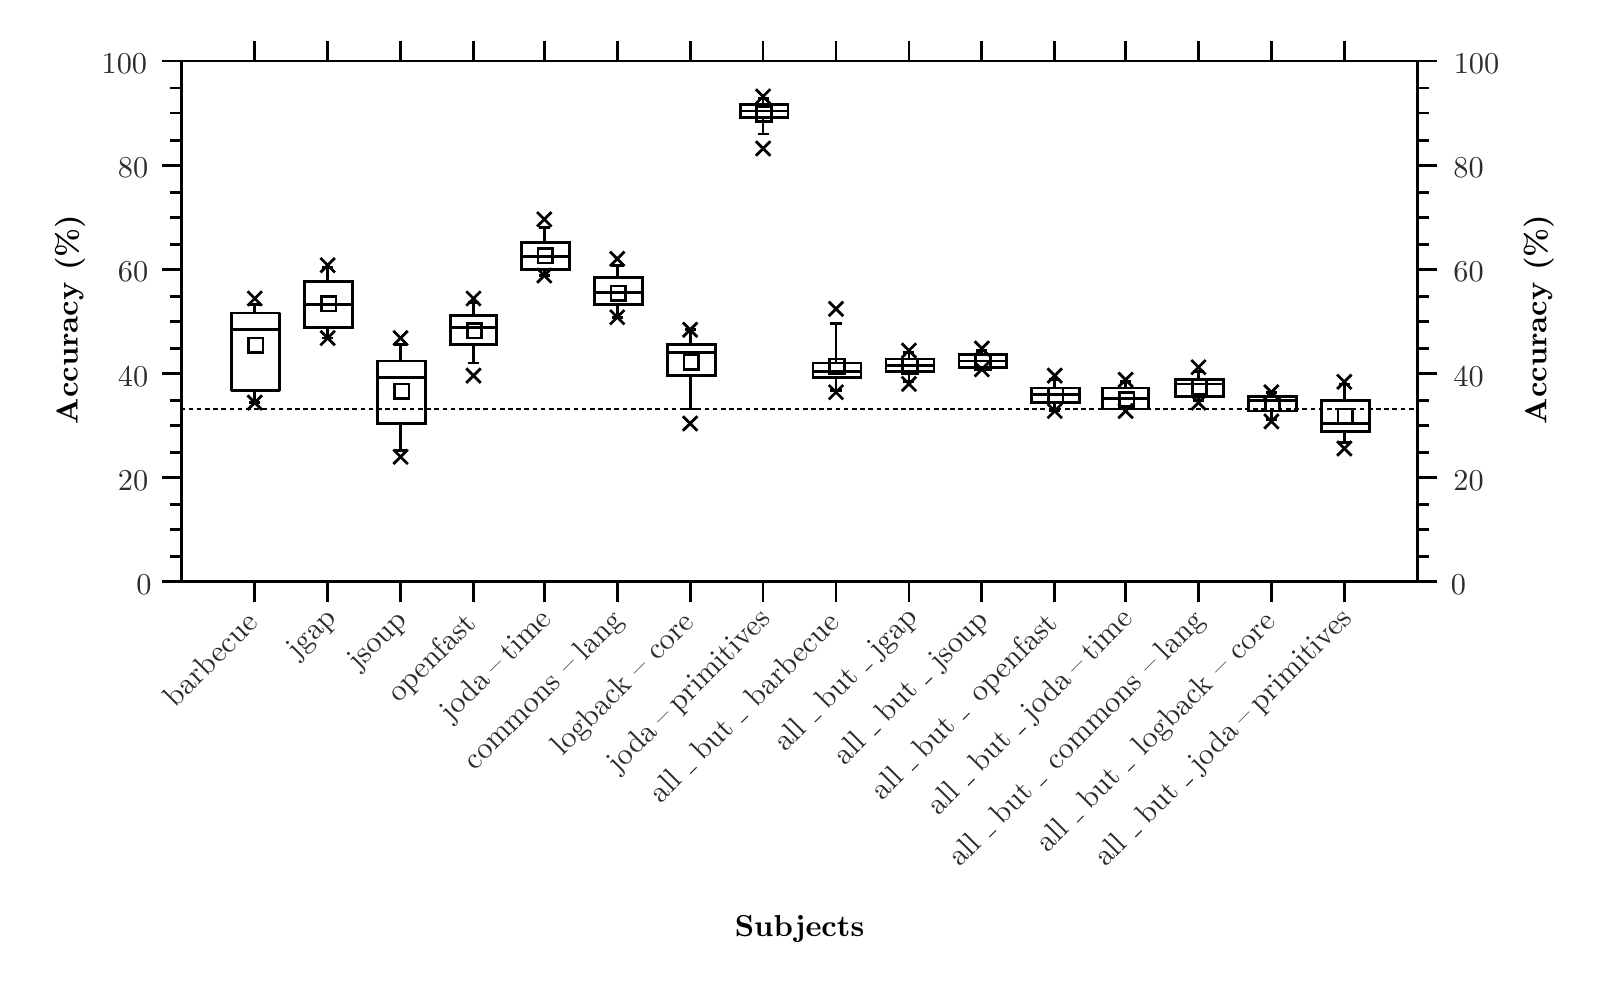
\begin{tikzpicture}{0pt}{0pt}{742pt}{452pt}
	\clip(0pt,452pt) -- (558.587pt,452pt) -- (558.587pt,111.729pt) -- (0pt,111.729pt) -- (0pt,452pt);
\begin{scope}
	\clip(55.7081pt,439.955pt) -- (502.126pt,439.955pt) -- (502.126pt,251.752pt) -- (55.7081pt,251.752pt) -- (55.7081pt,439.955pt);
	\color[rgb]{0,0,0}
	\draw[line width=1pt, line join=bevel, line cap=rect](73.7756pt,348.865pt) -- (91.0903pt,348.865pt) -- (91.0903pt,321.011pt) -- (73.7756pt,321.011pt) -- (73.7756pt,348.865pt);
	\color[rgb]{0,0,0}
	\draw[line width=1pt, line join=bevel, line cap=rect](80.5509pt,316.494pt) -- (83.5622pt,316.494pt);
	\draw[line width=1pt, line join=bevel, line cap=rect](80.5509pt,351.876pt) -- (83.5622pt,351.876pt);
	\draw[line width=1pt, line join=bevel, line cap=rect](82.0566pt,351.876pt) -- (82.0566pt,348.865pt);
	\draw[line width=1pt, line join=bevel, line cap=rect](82.0566pt,316.494pt) -- (82.0566pt,321.011pt);
	\draw[line width=1pt, line join=bevel, line cap=rect](73.7756pt,342.842pt) -- (90.3375pt,342.842pt);
	\draw[line width=1pt, line join=miter, line cap=rect](79.7981pt,318.752pt) -- (84.315pt,314.235pt);
	\draw[line width=1pt, line join=miter, line cap=rect](79.7981pt,314.235pt) -- (84.315pt,318.752pt);
	\draw[line width=1pt, line join=miter, line cap=rect](79.7981pt,356.393pt) -- (84.315pt,351.876pt);
	\draw[line width=1pt, line join=miter, line cap=rect](79.7981pt,351.876pt) -- (84.315pt,356.393pt);
	\draw[line width=1pt, line join=miter, line cap=rect](79.7981pt,339.831pt) -- (85.0678pt,339.831pt) -- (85.0678pt,334.561pt) -- (79.7981pt,334.561pt) -- (79.7981pt,339.831pt);
	\draw[line width=1pt, line join=miter, line cap=rect](100.124pt,360.157pt) -- (117.439pt,360.157pt) -- (117.439pt,343.595pt) -- (100.124pt,343.595pt) -- (100.124pt,360.157pt);
	\draw[line width=1pt, line join=miter, line cap=rect](106.899pt,339.831pt) -- (109.911pt,339.831pt);
	\draw[line width=1pt, line join=miter, line cap=rect](106.899pt,365.427pt) -- (109.911pt,365.427pt);
	\draw[line width=1pt, line join=miter, line cap=rect](108.405pt,365.427pt) -- (108.405pt,360.157pt);
	\draw[line width=1pt, line join=miter, line cap=rect](108.405pt,339.831pt) -- (108.405pt,343.595pt);
	\draw[line width=1pt, line join=miter, line cap=rect](100.124pt,351.876pt) -- (116.686pt,351.876pt);
	\draw[line width=1pt, line join=miter, line cap=rect](106.147pt,342.089pt) -- (110.663pt,337.572pt);
	\draw[line width=1pt, line join=miter, line cap=rect](106.147pt,337.572pt) -- (110.663pt,342.089pt);
	\draw[line width=1pt, line join=miter, line cap=rect](106.147pt,368.438pt) -- (110.663pt,363.921pt);
	\draw[line width=1pt, line join=miter, line cap=rect](106.147pt,363.921pt) -- (110.663pt,368.438pt);
	\draw[line width=1pt, line join=miter, line cap=rect](106.147pt,354.887pt) -- (111.416pt,354.887pt) -- (111.416pt,349.618pt) -- (106.147pt,349.618pt) -- (106.147pt,354.887pt);
	\draw[line width=1pt, line join=miter, line cap=rect](126.472pt,331.55pt) -- (143.787pt,331.55pt) -- (143.787pt,308.966pt) -- (126.472pt,308.966pt) -- (126.472pt,331.55pt);
	\draw[line width=1pt, line join=miter, line cap=rect](133.248pt,299.179pt) -- (136.259pt,299.179pt);
	\draw[line width=1pt, line join=miter, line cap=rect](133.248pt,337.572pt) -- (136.259pt,337.572pt);
	\draw[line width=1pt, line join=miter, line cap=rect](134.753pt,337.572pt) -- (134.753pt,331.55pt);
	\draw[line width=1pt, line join=miter, line cap=rect](134.753pt,299.179pt) -- (134.753pt,308.966pt);
	\draw[line width=1pt, line join=miter, line cap=rect](126.472pt,325.528pt) -- (143.034pt,325.528pt);
	\draw[line width=1pt, line join=miter, line cap=rect](132.495pt,299.179pt) -- (137.012pt,294.662pt);
	\draw[line width=1pt, line join=miter, line cap=rect](132.495pt,294.662pt) -- (137.012pt,299.179pt);
	\draw[line width=1pt, line join=miter, line cap=rect](132.495pt,342.089pt) -- (137.012pt,337.572pt);
	\draw[line width=1pt, line join=miter, line cap=rect](132.495pt,337.572pt) -- (137.012pt,342.089pt);
	\draw[line width=1pt, line join=miter, line cap=rect](132.495pt,323.269pt) -- (137.765pt,323.269pt) -- (137.765pt,317.999pt) -- (132.495pt,317.999pt) -- (132.495pt,323.269pt);
	\draw[line width=1pt, line join=miter, line cap=rect](152.821pt,348.112pt) -- (169.383pt,348.112pt) -- (169.383pt,337.572pt) -- (152.821pt,337.572pt) -- (152.821pt,348.112pt);
	\draw[line width=1pt, line join=miter, line cap=rect](159.596pt,330.797pt) -- (162.607pt,330.797pt);
	\draw[line width=1pt, line join=miter, line cap=rect](159.596pt,352.629pt) -- (162.607pt,352.629pt);
	\draw[line width=1pt, line join=miter, line cap=rect](161.102pt,352.629pt) -- (161.102pt,348.112pt);
	\draw[line width=1pt, line join=miter, line cap=rect](161.102pt,330.797pt) -- (161.102pt,337.572pt);
	\draw[line width=1pt, line join=miter, line cap=rect](152.821pt,343.595pt) -- (169.383pt,343.595pt);
	\draw[line width=1pt, line join=miter, line cap=rect](158.843pt,328.539pt) -- (163.36pt,324.022pt);
	\draw[line width=1pt, line join=miter, line cap=rect](158.843pt,324.022pt) -- (163.36pt,328.539pt);
	\draw[line width=1pt, line join=miter, line cap=rect](158.843pt,356.393pt) -- (163.36pt,351.876pt);
	\draw[line width=1pt, line join=miter, line cap=rect](158.843pt,351.876pt) -- (163.36pt,356.393pt);
	\draw[line width=1pt, line join=miter, line cap=rect](158.843pt,345.101pt) -- (164.113pt,345.101pt) -- (164.113pt,339.831pt) -- (158.843pt,339.831pt) -- (158.843pt,345.101pt);
	\draw[line width=1pt, line join=miter, line cap=rect](178.417pt,374.46pt) -- (195.731pt,374.46pt) -- (195.731pt,364.674pt) -- (178.417pt,364.674pt) -- (178.417pt,374.46pt);
	\draw[line width=1pt, line join=miter, line cap=rect](185.192pt,362.415pt) -- (188.203pt,362.415pt);
	\draw[line width=1pt, line join=miter, line cap=rect](185.192pt,379.73pt) -- (188.203pt,379.73pt);
	\draw[line width=1pt, line join=miter, line cap=rect](186.697pt,379.73pt) -- (186.697pt,374.46pt);
	\draw[line width=1pt, line join=miter, line cap=rect](186.697pt,362.415pt) -- (186.697pt,364.674pt);
	\draw[line width=1pt, line join=miter, line cap=rect](178.417pt,369.191pt) -- (194.978pt,369.191pt);
	\draw[line width=1pt, line join=miter, line cap=rect](184.439pt,364.674pt) -- (188.956pt,360.157pt);
	\draw[line width=1pt, line join=miter, line cap=rect](184.439pt,360.157pt) -- (188.956pt,364.674pt);
	\draw[line width=1pt, line join=miter, line cap=rect](184.439pt,385pt) -- (188.956pt,380.483pt);
	\draw[line width=1pt, line join=miter, line cap=rect](184.439pt,380.483pt) -- (188.956pt,385pt);
	\draw[line width=1pt, line join=miter, line cap=rect](184.439pt,372.202pt) -- (189.709pt,372.202pt) -- (189.709pt,366.932pt) -- (184.439pt,366.932pt) -- (184.439pt,372.202pt);
	\draw[line width=1pt, line join=miter, line cap=rect](204.765pt,361.663pt) -- (222.08pt,361.663pt) -- (222.08pt,351.876pt) -- (204.765pt,351.876pt) -- (204.765pt,361.663pt);
	\draw[line width=1pt, line join=miter, line cap=rect](211.54pt,347.359pt) -- (214.552pt,347.359pt);
	\draw[line width=1pt, line join=miter, line cap=rect](211.54pt,366.179pt) -- (214.552pt,366.179pt);
	\draw[line width=1pt, line join=miter, line cap=rect](213.046pt,366.179pt) -- (213.046pt,361.663pt);
	\draw[line width=1pt, line join=miter, line cap=rect](213.046pt,347.359pt) -- (213.046pt,351.876pt);
	\draw[line width=1pt, line join=miter, line cap=rect](204.765pt,356.393pt) -- (221.327pt,356.393pt);
	\draw[line width=1pt, line join=miter, line cap=rect](210.787pt,349.618pt) -- (215.304pt,345.101pt);
	\draw[line width=1pt, line join=miter, line cap=rect](210.787pt,345.101pt) -- (215.304pt,349.618pt);
	\draw[line width=1pt, line join=miter, line cap=rect](210.787pt,370.696pt) -- (215.304pt,366.179pt);
	\draw[line width=1pt, line join=miter, line cap=rect](210.787pt,366.179pt) -- (215.304pt,370.696pt);
	\draw[line width=1pt, line join=miter, line cap=rect](210.787pt,358.651pt) -- (216.057pt,358.651pt) -- (216.057pt,353.382pt) -- (210.787pt,353.382pt) -- (210.787pt,358.651pt);
	\draw[line width=1pt, line join=miter, line cap=rect](231.113pt,337.572pt) -- (248.428pt,337.572pt) -- (248.428pt,326.28pt) -- (231.113pt,326.28pt) -- (231.113pt,337.572pt);
	\draw[line width=1pt, line join=miter, line cap=rect](237.889pt,314.235pt) -- (240.9pt,314.235pt);
	\draw[line width=1pt, line join=miter, line cap=rect](237.889pt,342.842pt) -- (240.9pt,342.842pt);
	\draw[line width=1pt, line join=miter, line cap=rect](239.394pt,342.842pt) -- (239.394pt,337.572pt);
	\draw[line width=1pt, line join=miter, line cap=rect](239.394pt,314.235pt) -- (239.394pt,326.28pt);
	\draw[line width=1pt, line join=miter, line cap=rect](231.113pt,334.561pt) -- (247.675pt,334.561pt);
	\draw[line width=1pt, line join=miter, line cap=rect](237.136pt,311.224pt) -- (241.653pt,306.707pt);
	\draw[line width=1pt, line join=miter, line cap=rect](237.136pt,306.707pt) -- (241.653pt,311.224pt);
	\draw[line width=1pt, line join=miter, line cap=rect](237.136pt,345.101pt) -- (241.653pt,340.584pt);
	\draw[line width=1pt, line join=miter, line cap=rect](237.136pt,340.584pt) -- (241.653pt,345.101pt);
	\draw[line width=1pt, line join=miter, line cap=rect](237.136pt,333.808pt) -- (242.406pt,333.808pt) -- (242.406pt,328.539pt) -- (237.136pt,328.539pt) -- (237.136pt,333.808pt);
	\draw[line width=1pt, line join=miter, line cap=rect](257.462pt,424.146pt) -- (274.777pt,424.146pt) -- (274.777pt,419.629pt) -- (257.462pt,419.629pt) -- (257.462pt,424.146pt);
	\draw[line width=1pt, line join=miter, line cap=rect](264.237pt,413.607pt) -- (267.248pt,413.607pt);
	\draw[line width=1pt, line join=miter, line cap=rect](264.237pt,426.404pt) -- (267.248pt,426.404pt);
	\draw[line width=1pt, line join=miter, line cap=rect](265.743pt,426.404pt) -- (265.743pt,424.146pt);
	\draw[line width=1pt, line join=miter, line cap=rect](265.743pt,413.607pt) -- (265.743pt,419.629pt);
	\draw[line width=1pt, line join=miter, line cap=rect](257.462pt,421.887pt) -- (274.024pt,421.887pt);
	\draw[line width=1pt, line join=miter, line cap=rect](263.484pt,410.595pt) -- (268.001pt,406.078pt);
	\draw[line width=1pt, line join=miter, line cap=rect](263.484pt,406.078pt) -- (268.001pt,410.595pt);
	\draw[line width=1pt, line join=miter, line cap=rect](263.484pt,429.416pt) -- (268.001pt,424.899pt);
	\draw[line width=1pt, line join=miter, line cap=rect](263.484pt,424.899pt) -- (268.001pt,429.416pt);
	\draw[line width=1pt, line join=miter, line cap=rect](263.484pt,423.393pt) -- (268.754pt,423.393pt) -- (268.754pt,418.123pt) -- (263.484pt,418.123pt) -- (263.484pt,423.393pt);
	\draw[line width=1pt, line join=miter, line cap=rect](283.81pt,330.797pt) -- (301.125pt,330.797pt) -- (301.125pt,325.528pt) -- (283.81pt,325.528pt) -- (283.81pt,330.797pt);
	\draw[line width=1pt, line join=miter, line cap=rect](290.586pt,321.011pt) -- (293.597pt,321.011pt);
	\draw[line width=1pt, line join=miter, line cap=rect](290.586pt,345.101pt) -- (293.597pt,345.101pt);
	\draw[line width=1pt, line join=miter, line cap=rect](292.091pt,345.101pt) -- (292.091pt,330.797pt);
	\draw[line width=1pt, line join=miter, line cap=rect](292.091pt,321.011pt) -- (292.091pt,325.528pt);
	\draw[line width=1pt, line join=miter, line cap=rect](283.81pt,327.786pt) -- (300.372pt,327.786pt);
	\draw[line width=1pt, line join=miter, line cap=rect](289.833pt,322.516pt) -- (294.35pt,317.999pt);
	\draw[line width=1pt, line join=miter, line cap=rect](289.833pt,317.999pt) -- (294.35pt,322.516pt);
	\draw[line width=1pt, line join=miter, line cap=rect](289.833pt,352.629pt) -- (294.35pt,348.112pt);
	\draw[line width=1pt, line join=miter, line cap=rect](289.833pt,348.112pt) -- (294.35pt,352.629pt);
	\draw[line width=1pt, line join=miter, line cap=rect](289.833pt,332.303pt) -- (295.103pt,332.303pt) -- (295.103pt,327.033pt) -- (289.833pt,327.033pt) -- (289.833pt,332.303pt);
	\draw[line width=1pt, line join=miter, line cap=rect](310.159pt,332.303pt) -- (327.473pt,332.303pt) -- (327.473pt,327.786pt) -- (310.159pt,327.786pt) -- (310.159pt,332.303pt);
	\draw[line width=1pt, line join=miter, line cap=rect](316.934pt,324.022pt) -- (319.945pt,324.022pt);
	\draw[line width=1pt, line join=miter, line cap=rect](316.934pt,334.561pt) -- (319.945pt,334.561pt);
	\draw[line width=1pt, line join=miter, line cap=rect](318.44pt,334.561pt) -- (318.44pt,332.303pt);
	\draw[line width=1pt, line join=miter, line cap=rect](318.44pt,324.022pt) -- (318.44pt,327.786pt);
	\draw[line width=1pt, line join=miter, line cap=rect](310.159pt,330.044pt) -- (326.721pt,330.044pt);
	\draw[line width=1pt, line join=miter, line cap=rect](316.181pt,325.528pt) -- (320.698pt,321.011pt);
	\draw[line width=1pt, line join=miter, line cap=rect](316.181pt,321.011pt) -- (320.698pt,325.528pt);
	\draw[line width=1pt, line join=miter, line cap=rect](316.181pt,337.572pt) -- (320.698pt,333.056pt);
	\draw[line width=1pt, line join=miter, line cap=rect](316.181pt,333.056pt) -- (320.698pt,337.572pt);
	\draw[line width=1pt, line join=miter, line cap=rect](316.181pt,332.303pt) -- (321.451pt,332.303pt) -- (321.451pt,327.033pt) -- (316.181pt,327.033pt) -- (316.181pt,332.303pt);
	\draw[line width=1pt, line join=miter, line cap=rect](336.507pt,333.808pt) -- (353.822pt,333.808pt) -- (353.822pt,329.292pt) -- (336.507pt,329.292pt) -- (336.507pt,333.808pt);
	\draw[line width=1pt, line join=miter, line cap=rect](343.282pt,328.539pt) -- (346.294pt,328.539pt);
	\draw[line width=1pt, line join=miter, line cap=rect](343.282pt,335.314pt) -- (346.294pt,335.314pt);
	\draw[line width=1pt, line join=miter, line cap=rect](344.788pt,335.314pt) -- (344.788pt,333.808pt);
	\draw[line width=1pt, line join=miter, line cap=rect](344.788pt,328.539pt) -- (344.788pt,329.292pt);
	\draw[line width=1pt, line join=miter, line cap=rect](336.507pt,331.55pt) -- (353.069pt,331.55pt);
	\draw[line width=1pt, line join=miter, line cap=rect](342.53pt,330.797pt) -- (347.047pt,326.28pt);
	\draw[line width=1pt, line join=miter, line cap=rect](342.53pt,326.28pt) -- (347.047pt,330.797pt);
	\draw[line width=1pt, line join=miter, line cap=rect](342.53pt,338.325pt) -- (347.047pt,333.808pt);
	\draw[line width=1pt, line join=miter, line cap=rect](342.53pt,333.808pt) -- (347.047pt,338.325pt);
	\draw[line width=1pt, line join=miter, line cap=rect](342.53pt,333.808pt) -- (347.799pt,333.808pt) -- (347.799pt,328.539pt) -- (342.53pt,328.539pt) -- (342.53pt,333.808pt);
	\draw[line width=1pt, line join=miter, line cap=rect](362.856pt,321.763pt) -- (380.17pt,321.763pt) -- (380.17pt,316.494pt) -- (362.856pt,316.494pt) -- (362.856pt,321.763pt);
	\draw[line width=1pt, line join=miter, line cap=rect](369.631pt,313.482pt) -- (372.642pt,313.482pt);
	\draw[line width=1pt, line join=miter, line cap=rect](369.631pt,324.775pt) -- (372.642pt,324.775pt);
	\draw[line width=1pt, line join=miter, line cap=rect](371.137pt,324.775pt) -- (371.137pt,321.763pt);
	\draw[line width=1pt, line join=miter, line cap=rect](371.137pt,313.482pt) -- (371.137pt,316.494pt);
	\draw[line width=1pt, line join=miter, line cap=rect](362.856pt,319.505pt) -- (379.418pt,319.505pt);
	\draw[line width=1pt, line join=miter, line cap=rect](368.878pt,315.741pt) -- (373.395pt,311.224pt);
	\draw[line width=1pt, line join=miter, line cap=rect](368.878pt,311.224pt) -- (373.395pt,315.741pt);
	\draw[line width=1pt, line join=miter, line cap=rect](368.878pt,328.539pt) -- (373.395pt,324.022pt);
	\draw[line width=1pt, line join=miter, line cap=rect](368.878pt,324.022pt) -- (373.395pt,328.539pt);
	\draw[line width=1pt, line join=miter, line cap=rect](368.878pt,321.763pt) -- (374.148pt,321.763pt) -- (374.148pt,316.494pt) -- (368.878pt,316.494pt) -- (368.878pt,321.763pt);
	\draw[line width=1pt, line join=miter, line cap=rect](388.451pt,321.763pt) -- (405.013pt,321.763pt) -- (405.013pt,314.235pt) -- (388.451pt,314.235pt) -- (388.451pt,321.763pt);
	\draw[line width=1pt, line join=miter, line cap=rect](395.227pt,314.235pt) -- (398.238pt,314.235pt);
	\draw[line width=1pt, line join=miter, line cap=rect](395.227pt,324.022pt) -- (398.238pt,324.022pt);
	\draw[line width=1pt, line join=miter, line cap=rect](396.732pt,324.022pt) -- (396.732pt,321.763pt);

	\draw[line width=1pt, line join=miter, line cap=rect](388.451pt,317.999pt) -- (405.013pt,317.999pt);
	\draw[line width=1pt, line join=miter, line cap=rect](394.474pt,315.741pt) -- (398.991pt,311.224pt);
	\draw[line width=1pt, line join=miter, line cap=rect](394.474pt,311.224pt) -- (398.991pt,315.741pt);
	\draw[line width=1pt, line join=miter, line cap=rect](394.474pt,327.033pt) -- (398.991pt,322.516pt);
	\draw[line width=1pt, line join=miter, line cap=rect](394.474pt,322.516pt) -- (398.991pt,327.033pt);
	\draw[line width=1pt, line join=miter, line cap=rect](394.474pt,320.258pt) -- (399.743pt,320.258pt) -- (399.743pt,314.988pt) -- (394.474pt,314.988pt) -- (394.474pt,320.258pt);
	\draw[line width=1pt, line join=miter, line cap=rect](414.8pt,324.775pt) -- (432.114pt,324.775pt) -- (432.114pt,318.752pt) -- (414.8pt,318.752pt) -- (414.8pt,324.775pt);
	\draw[line width=1pt, line join=miter, line cap=rect](421.575pt,317.247pt) -- (424.586pt,317.247pt);
	\draw[line width=1pt, line join=miter, line cap=rect](421.575pt,327.786pt) -- (424.586pt,327.786pt);
	\draw[line width=1pt, line join=miter, line cap=rect](423.081pt,327.786pt) -- (423.081pt,324.775pt);
	\draw[line width=1pt, line join=miter, line cap=rect](423.081pt,317.247pt) -- (423.081pt,318.752pt);
	\draw[line width=1pt, line join=miter, line cap=rect](414.8pt,323.269pt) -- (431.362pt,323.269pt);
	\draw[line width=1pt, line join=miter, line cap=rect](420.822pt,318.752pt) -- (425.339pt,314.235pt);
	\draw[line width=1pt, line join=miter, line cap=rect](420.822pt,314.235pt) -- (425.339pt,318.752pt);
	\draw[line width=1pt, line join=miter, line cap=rect](420.822pt,331.55pt) -- (425.339pt,327.033pt);
	\draw[line width=1pt, line join=miter, line cap=rect](420.822pt,327.033pt) -- (425.339pt,331.55pt);
	\draw[line width=1pt, line join=miter, line cap=rect](420.822pt,324.775pt) -- (426.092pt,324.775pt) -- (426.092pt,319.505pt) -- (420.822pt,319.505pt) -- (420.822pt,324.775pt);
	\draw[line width=1pt, line join=miter, line cap=rect](441.148pt,318.752pt) -- (458.463pt,318.752pt) -- (458.463pt,313.482pt) -- (441.148pt,313.482pt) -- (441.148pt,318.752pt);
	\draw[line width=1pt, line join=miter, line cap=rect](447.923pt,310.471pt) -- (450.935pt,310.471pt);
	\draw[line width=1pt, line join=miter, line cap=rect](447.923pt,320.258pt) -- (450.935pt,320.258pt);
	\draw[line width=1pt, line join=miter, line cap=rect](449.429pt,320.258pt) -- (449.429pt,318.752pt);
	\draw[line width=1pt, line join=miter, line cap=rect](449.429pt,310.471pt) -- (449.429pt,313.482pt);
	\draw[line width=1pt, line join=miter, line cap=rect](441.148pt,317.247pt) -- (457.71pt,317.247pt);
	\draw[line width=1pt, line join=miter, line cap=rect](447.171pt,311.977pt) -- (451.688pt,307.46pt);
	\draw[line width=1pt, line join=miter, line cap=rect](447.171pt,307.46pt) -- (451.688pt,311.977pt);
	\draw[line width=1pt, line join=miter, line cap=rect](447.171pt,322.516pt) -- (451.688pt,317.999pt);
	\draw[line width=1pt, line join=miter, line cap=rect](447.171pt,317.999pt) -- (451.688pt,322.516pt);
	\draw[line width=1pt, line join=miter, line cap=rect](447.171pt,318.752pt) -- (452.44pt,318.752pt) -- (452.44pt,313.482pt) -- (447.171pt,313.482pt) -- (447.171pt,318.752pt);
	\draw[line width=1pt, line join=miter, line cap=rect](467.497pt,317.247pt) -- (484.811pt,317.247pt) -- (484.811pt,305.954pt) -- (467.497pt,305.954pt) -- (467.497pt,317.247pt);
	\draw[line width=1pt, line join=miter, line cap=rect](474.272pt,302.19pt) -- (477.283pt,302.19pt);
	\draw[line width=1pt, line join=miter, line cap=rect](474.272pt,323.269pt) -- (477.283pt,323.269pt);
	\draw[line width=1pt, line join=miter, line cap=rect](475.777pt,323.269pt) -- (475.777pt,317.247pt);
	\draw[line width=1pt, line join=miter, line cap=rect](475.777pt,302.19pt) -- (475.777pt,305.954pt);
	\draw[line width=1pt, line join=miter, line cap=rect](467.497pt,308.966pt) -- (484.058pt,308.966pt);
	\draw[line width=1pt, line join=miter, line cap=rect](473.519pt,302.19pt) -- (478.036pt,297.673pt);
	\draw[line width=1pt, line join=miter, line cap=rect](473.519pt,297.673pt) -- (478.036pt,302.19pt);
	\draw[line width=1pt, line join=miter, line cap=rect](473.519pt,326.28pt) -- (478.036pt,321.763pt);
	\draw[line width=1pt, line join=miter, line cap=rect](473.519pt,321.763pt) -- (478.036pt,326.28pt);
	\draw[line width=1pt, line join=miter, line cap=rect](473.519pt,314.235pt) -- (478.789pt,314.235pt) -- (478.789pt,308.966pt) -- (473.519pt,308.966pt) -- (473.519pt,314.235pt);


	\draw[line width=1pt, dash pattern=on 0.024cm off 0.08cm, dash phase=0pt, line join=miter, line cap=rect](55.7081pt,314.235pt) -- (528.474pt,314.235pt);
\end{scope}
\begin{scope}
	\color[rgb]{0,0,0}
	\pgftext[center, base, at={\pgfpoint{18.0675pt}{346.606pt}},rotate=90]{\fontsize{11}{0}\selectfont{\textbf{Accuracy (\%)}}}
	\color[rgb]{0.172549,0.172549,0.172549}
	\pgftext[center, base, at={\pgfpoint{42.0163pt}{247.235pt}}]{\fontsize{11}{0}\selectfont{0}}
	\pgftext[center, base, at={\pgfpoint{38.1111pt}{284.876pt}}]{\fontsize{11}{0}\selectfont{20}}
	\pgftext[center, base, at={\pgfpoint{38.1111pt}{322.516pt}}]{\fontsize{11}{0}\selectfont{40}}
	\pgftext[center, base, at={\pgfpoint{38.1111pt}{360.157pt}}]{\fontsize{11}{0}\selectfont{60}}
	\pgftext[center, base, at={\pgfpoint{38.1111pt}{397.798pt}}]{\fontsize{11}{0}\selectfont{80}}
	\pgftext[center, base, at={\pgfpoint{34.9587pt}{435.438pt}}]{\fontsize{11}{0}\selectfont{100}}
	\color[rgb]{0,0,0}
	\draw[line width=1pt, line join=bevel, line cap=rect](55.7081pt,260.786pt) -- (51.9441pt,260.786pt);
	\draw[line width=1pt, line join=bevel, line cap=rect](55.7081pt,279.606pt) -- (51.9441pt,279.606pt);
	\draw[line width=1pt, line join=bevel, line cap=rect](55.7081pt,298.426pt) -- (51.9441pt,298.426pt);
	\draw[line width=1pt, line join=bevel, line cap=rect](55.7081pt,317.247pt) -- (51.9441pt,317.247pt);
	\draw[line width=1pt, line join=bevel, line cap=rect](55.7081pt,336.067pt) -- (51.9441pt,336.067pt);
	\draw[line width=1pt, line join=bevel, line cap=rect](55.7081pt,354.887pt) -- (51.9441pt,354.887pt);
	\draw[line width=1pt, line join=bevel, line cap=rect](55.7081pt,373.707pt) -- (51.9441pt,373.707pt);
	\draw[line width=1pt, line join=bevel, line cap=rect](55.7081pt,392.528pt) -- (51.9441pt,392.528pt);
	\draw[line width=1pt, line join=bevel, line cap=rect](55.7081pt,411.348pt) -- (51.9441pt,411.348pt);
	\draw[line width=1pt, line join=bevel, line cap=rect](55.7081pt,430.168pt) -- (51.9441pt,430.168pt);
	\draw[line width=1pt, line join=bevel, line cap=rect](55.7081pt,270.572pt) -- (51.9441pt,270.572pt);
	\draw[line width=1pt, line join=bevel, line cap=rect](55.7081pt,308.213pt) -- (51.9441pt,308.213pt);
	\draw[line width=1pt, line join=bevel, line cap=rect](55.7081pt,345.853pt) -- (51.9441pt,345.853pt);
	\draw[line width=1pt, line join=bevel, line cap=rect](55.7081pt,383.494pt) -- (51.9441pt,383.494pt);
	\draw[line width=1pt, line join=bevel, line cap=rect](55.7081pt,421.135pt) -- (51.9441pt,421.135pt);
	\draw[line width=1pt, line join=bevel, line cap=rect](55.7081pt,251.752pt) -- (48.9328pt,251.752pt);
	\draw[line width=1pt, line join=bevel, line cap=rect](55.7081pt,289.393pt) -- (48.9328pt,289.393pt);
	\draw[line width=1pt, line join=bevel, line cap=rect](55.7081pt,327.033pt) -- (48.9328pt,327.033pt);
	\draw[line width=1pt, line join=bevel, line cap=rect](55.7081pt,364.674pt) -- (48.9328pt,364.674pt);
	\draw[line width=1pt, line join=bevel, line cap=rect](55.7081pt,402.314pt) -- (48.9328pt,402.314pt);
	\draw[line width=1pt, line join=bevel, line cap=rect](55.7081pt,439.955pt) -- (48.9328pt,439.955pt);
	\draw[line width=1pt, line join=bevel, line cap=rect](55.7081pt,439.955pt) -- (55.7081pt,251.752pt);
	\pgftext[center, base, at={\pgfpoint{548.8pt}{346.606pt}},rotate=90]{\fontsize{11}{0}\selectfont{\textbf{Accuracy (\%)}}}
	\color[rgb]{0.172549,0.172549,0.172549}
	\pgftext[center, base, at={\pgfpoint{517.041pt}{247.235pt}}]{\fontsize{11}{0}\selectfont{0}}
	\pgftext[center, base, at={\pgfpoint{520.664pt}{284.876pt}}]{\fontsize{11}{0}\selectfont{20}}
	\pgftext[center, base, at={\pgfpoint{520.664pt}{322.516pt}}]{\fontsize{11}{0}\selectfont{40}}
	\pgftext[center, base, at={\pgfpoint{520.664pt}{360.157pt}}]{\fontsize{11}{0}\selectfont{60}}
	\pgftext[center, base, at={\pgfpoint{520.664pt}{397.798pt}}]{\fontsize{11}{0}\selectfont{80}}
	\pgftext[center, base, at={\pgfpoint{523.534pt}{435.438pt}}]{\fontsize{11}{0}\selectfont{100}}
	\color[rgb]{0,0,0}
	\draw[line width=1pt, line join=bevel, line cap=rect](502.126pt,260.786pt) -- (505.89pt,260.786pt);
	\draw[line width=1pt, line join=bevel, line cap=rect](502.126pt,279.606pt) -- (505.89pt,279.606pt);
	\draw[line width=1pt, line join=bevel, line cap=rect](502.126pt,298.426pt) -- (505.89pt,298.426pt);
	\draw[line width=1pt, line join=bevel, line cap=rect](502.126pt,317.247pt) -- (505.89pt,317.247pt);
	\draw[line width=1pt, line join=bevel, line cap=rect](502.126pt,336.067pt) -- (505.89pt,336.067pt);
	\draw[line width=1pt, line join=bevel, line cap=rect](502.126pt,354.887pt) -- (505.89pt,354.887pt);
	\draw[line width=1pt, line join=bevel, line cap=rect](502.126pt,373.707pt) -- (505.89pt,373.707pt);
	\draw[line width=1pt, line join=bevel, line cap=rect](502.126pt,392.528pt) -- (505.89pt,392.528pt);
	\draw[line width=1pt, line join=bevel, line cap=rect](502.126pt,411.348pt) -- (505.89pt,411.348pt);
	\draw[line width=1pt, line join=bevel, line cap=rect](502.126pt,430.168pt) -- (505.89pt,430.168pt);
	\draw[line width=1pt, line join=bevel, line cap=rect](502.126pt,270.572pt) -- (505.89pt,270.572pt);
	\draw[line width=1pt, line join=bevel, line cap=rect](502.126pt,308.213pt) -- (505.89pt,308.213pt);
	\draw[line width=1pt, line join=bevel, line cap=rect](502.126pt,345.853pt) -- (505.89pt,345.853pt);
	\draw[line width=1pt, line join=bevel, line cap=rect](502.126pt,383.494pt) -- (505.89pt,383.494pt);
	\draw[line width=1pt, line join=bevel, line cap=rect](502.126pt,421.135pt) -- (505.89pt,421.135pt);
	\draw[line width=1pt, line join=bevel, line cap=rect](502.126pt,251.752pt) -- (508.901pt,251.752pt);
	\draw[line width=1pt, line join=bevel, line cap=rect](502.126pt,289.393pt) -- (508.901pt,289.393pt);
	\draw[line width=1pt, line join=bevel, line cap=rect](502.126pt,327.033pt) -- (508.901pt,327.033pt);
	\draw[line width=1pt, line join=bevel, line cap=rect](502.126pt,364.674pt) -- (508.901pt,364.674pt);
	\draw[line width=1pt, line join=bevel, line cap=rect](502.126pt,402.314pt) -- (508.901pt,402.314pt);
	\draw[line width=1pt, line join=bevel, line cap=rect](502.126pt,439.955pt) -- (508.901pt,439.955pt);
	\draw[line width=1pt, line join=bevel, line cap=rect](502.126pt,439.955pt) -- (502.126pt,251.752pt);
	\pgftext[center, base, at={\pgfpoint{278.917pt}{123.774pt}}]{\fontsize{11}{0}\selectfont{\textbf{Subjects}}}
	\color[rgb]{0.172549,0.172549,0.172549}
	\pgftext[center, base, at={\pgfpoint{68.4991pt}{221.267pt}},rotate=45]{\fontsize{11}{0}\selectfont{barbecue}}
	\pgftext[center, base, at={\pgfpoint{104.654pt}{231.073pt}},rotate=45]{\fontsize{11}{0}\selectfont{jgap}}
	\pgftext[center, base, at={\pgfpoint{128.445pt}{228.516pt}},rotate=45]{\fontsize{11}{0}\selectfont{jsoup}}
	\pgftext[center, base, at={\pgfpoint{148.222pt}{221.945pt}},rotate=45]{\fontsize{11}{0}\selectfont{openfast}}
	\pgftext[center, base, at={\pgfpoint{160.198pt}{208.325pt}},rotate=45]{\fontsize{11}{0}\selectfont{joda}}
	\pgftext[center, base, at={\pgfpoint{171.111pt}{219.238pt}},rotate=45]{\fontsize{11}{0}\selectfont{--}}
	\pgftext[center, base, at={\pgfpoint{182.11pt}{230.238pt}},rotate=45]{\fontsize{11}{0}\selectfont{time}}
	\pgftext[center, base, at={\pgfpoint{177.272pt}{199.051pt}},rotate=45]{\fontsize{11}{0}\selectfont{commons}}
	\pgftext[center, base, at={\pgfpoint{197.542pt}{219.321pt}},rotate=45]{\fontsize{11}{0}\selectfont{--}}
	\pgftext[center, base, at={\pgfpoint{208.405pt}{230.184pt}},rotate=45]{\fontsize{11}{0}\selectfont{lang}}
	\pgftext[center, base, at={\pgfpoint{205.896pt}{201.326pt}},rotate=45]{\fontsize{11}{0}\selectfont{logback}}
	\pgftext[center, base, at={\pgfpoint{223.117pt}{218.547pt}},rotate=45]{\fontsize{11}{0}\selectfont{--}}
	\pgftext[center, base, at={\pgfpoint{234.342pt}{229.772pt}},rotate=45]{\fontsize{11}{0}\selectfont{core}}
	\pgftext[center, base, at={\pgfpoint{220.612pt}{189.694pt}},rotate=45]{\fontsize{11}{0}\selectfont{joda}}
	\pgftext[center, base, at={\pgfpoint{231.525pt}{200.607pt}},rotate=45]{\fontsize{11}{0}\selectfont{--}}
	\pgftext[center, base, at={\pgfpoint{252.027pt}{221.109pt}},rotate=45]{\fontsize{11}{0}\selectfont{primitives}}
	\pgftext[center, base, at={\pgfpoint{232.684pt}{175.417pt}},rotate=45]{\fontsize{11}{0}\selectfont{all}}
	\pgftext[center, base, at={\pgfpoint{240.498pt}{183.231pt}},rotate=45]{\fontsize{11}{0}\selectfont{\_}}
	\pgftext[center, base, at={\pgfpoint{249.743pt}{192.476pt}},rotate=45]{\fontsize{11}{0}\selectfont{but}}
	\pgftext[center, base, at={\pgfpoint{258.988pt}{201.721pt}},rotate=45]{\fontsize{11}{0}\selectfont{\_}}
	\pgftext[center, base, at={\pgfpoint{278.584pt}{221.317pt}},rotate=45]{\fontsize{11}{0}\selectfont{barbecue}}
	\pgftext[center, base, at={\pgfpoint{277.663pt}{194.048pt}},rotate=45]{\fontsize{11}{0}\selectfont{all}}
	\pgftext[center, base, at={\pgfpoint{285.478pt}{201.862pt}},rotate=45]{\fontsize{11}{0}\selectfont{\_}}
	\pgftext[center, base, at={\pgfpoint{294.722pt}{211.107pt}},rotate=45]{\fontsize{11}{0}\selectfont{but}}
	\pgftext[center, base, at={\pgfpoint{303.967pt}{220.352pt}},rotate=45]{\fontsize{11}{0}\selectfont{\_}}
	\pgftext[center, base, at={\pgfpoint{314.738pt}{231.123pt}},rotate=45]{\fontsize{11}{0}\selectfont{jgap}}
	\pgftext[center, base, at={\pgfpoint{299.221pt}{189.257pt}},rotate=45]{\fontsize{11}{0}\selectfont{all}}
	\pgftext[center, base, at={\pgfpoint{307.035pt}{197.072pt}},rotate=45]{\fontsize{11}{0}\selectfont{\_}}
	\pgftext[center, base, at={\pgfpoint{316.28pt}{206.317pt}},rotate=45]{\fontsize{11}{0}\selectfont{but}}
	\pgftext[center, base, at={\pgfpoint{325.525pt}{215.561pt}},rotate=45]{\fontsize{11}{0}\selectfont{\_}}
	\pgftext[center, base, at={\pgfpoint{338.529pt}{228.566pt}},rotate=45]{\fontsize{11}{0}\selectfont{jsoup}}
	\pgftext[center, base, at={\pgfpoint{312.794pt}{176.482pt}},rotate=45]{\fontsize{11}{0}\selectfont{all}}
	\pgftext[center, base, at={\pgfpoint{320.608pt}{184.296pt}},rotate=45]{\fontsize{11}{0}\selectfont{\_}}
	\pgftext[center, base, at={\pgfpoint{329.853pt}{193.541pt}},rotate=45]{\fontsize{11}{0}\selectfont{but}}
	\pgftext[center, base, at={\pgfpoint{339.098pt}{202.786pt}},rotate=45]{\fontsize{11}{0}\selectfont{\_}}
	\pgftext[center, base, at={\pgfpoint{358.307pt}{221.995pt}},rotate=45]{\fontsize{11}{0}\selectfont{openfast}}
	\pgftext[center, base, at={\pgfpoint{333.066pt}{171.159pt}},rotate=45]{\fontsize{11}{0}\selectfont{all}}
	\pgftext[center, base, at={\pgfpoint{340.88pt}{178.973pt}},rotate=45]{\fontsize{11}{0}\selectfont{\_}}
	\pgftext[center, base, at={\pgfpoint{350.125pt}{188.218pt}},rotate=45]{\fontsize{11}{0}\selectfont{but}}
	\pgftext[center, base, at={\pgfpoint{359.37pt}{197.463pt}},rotate=45]{\fontsize{11}{0}\selectfont{\_}}
	\pgftext[center, base, at={\pgfpoint{370.283pt}{208.375pt}},rotate=45]{\fontsize{11}{0}\selectfont{joda}}
	\pgftext[center, base, at={\pgfpoint{381.195pt}{219.288pt}},rotate=45]{\fontsize{11}{0}\selectfont{--}}
	\pgftext[center, base, at={\pgfpoint{392.195pt}{230.287pt}},rotate=45]{\fontsize{11}{0}\selectfont{time}}
	\pgftext[center, base, at={\pgfpoint{340.783pt}{152.527pt}},rotate=45]{\fontsize{11}{0}\selectfont{all}}
	\pgftext[center, base, at={\pgfpoint{348.598pt}{160.342pt}},rotate=45]{\fontsize{11}{0}\selectfont{\_}}
	\pgftext[center, base, at={\pgfpoint{357.842pt}{169.587pt}},rotate=45]{\fontsize{11}{0}\selectfont{but}}
	\pgftext[center, base, at={\pgfpoint{367.087pt}{178.831pt}},rotate=45]{\fontsize{11}{0}\selectfont{\_}}
	\pgftext[center, base, at={\pgfpoint{387.357pt}{199.101pt}},rotate=45]{\fontsize{11}{0}\selectfont{commons}}
	\pgftext[center, base, at={\pgfpoint{407.627pt}{219.371pt}},rotate=45]{\fontsize{11}{0}\selectfont{--}}
	\pgftext[center, base, at={\pgfpoint{418.489pt}{230.233pt}},rotate=45]{\fontsize{11}{0}\selectfont{lang}}
	\pgftext[center, base, at={\pgfpoint{372.455pt}{157.851pt}},rotate=45]{\fontsize{11}{0}\selectfont{all}}
	\pgftext[center, base, at={\pgfpoint{380.269pt}{165.665pt}},rotate=45]{\fontsize{11}{0}\selectfont{\_}}
	\pgftext[center, base, at={\pgfpoint{389.514pt}{174.91pt}},rotate=45]{\fontsize{11}{0}\selectfont{but}}
	\pgftext[center, base, at={\pgfpoint{398.759pt}{184.155pt}},rotate=45]{\fontsize{11}{0}\selectfont{\_}}
	\pgftext[center, base, at={\pgfpoint{415.98pt}{201.376pt}},rotate=45]{\fontsize{11}{0}\selectfont{logback}}
	\pgftext[center, base, at={\pgfpoint{433.202pt}{218.597pt}},rotate=45]{\fontsize{11}{0}\selectfont{--}}
	\pgftext[center, base, at={\pgfpoint{444.426pt}{229.822pt}},rotate=45]{\fontsize{11}{0}\selectfont{core}}
	\pgftext[center, base, at={\pgfpoint{393.48pt}{152.527pt}},rotate=45]{\fontsize{11}{0}\selectfont{all}}
	\pgftext[center, base, at={\pgfpoint{401.294pt}{160.342pt}},rotate=45]{\fontsize{11}{0}\selectfont{\_}}
	\pgftext[center, base, at={\pgfpoint{410.539pt}{169.587pt}},rotate=45]{\fontsize{11}{0}\selectfont{but}}
	\pgftext[center, base, at={\pgfpoint{419.784pt}{178.831pt}},rotate=45]{\fontsize{11}{0}\selectfont{\_}}
	\pgftext[center, base, at={\pgfpoint{430.697pt}{189.744pt}},rotate=45]{\fontsize{11}{0}\selectfont{joda}}
	\pgftext[center, base, at={\pgfpoint{441.609pt}{200.656pt}},rotate=45]{\fontsize{11}{0}\selectfont{--}}
	\pgftext[center, base, at={\pgfpoint{462.112pt}{221.159pt}},rotate=45]{\fontsize{11}{0}\selectfont{primitives}}
	\color[rgb]{0,0,0}
	\draw[line width=1pt, line join=bevel, line cap=rect](82.0566pt,251.752pt) -- (82.0566pt,244.977pt);
	\draw[line width=1pt, line join=bevel, line cap=rect](108.405pt,251.752pt) -- (108.405pt,244.977pt);
	\draw[line width=1pt, line join=bevel, line cap=rect](134.753pt,251.752pt) -- (134.753pt,244.977pt);
	\draw[line width=1pt, line join=bevel, line cap=rect](161.102pt,251.752pt) -- (161.102pt,244.977pt);
	\draw[line width=1pt, line join=bevel, line cap=rect](186.697pt,251.752pt) -- (186.697pt,244.977pt);
	\draw[line width=1pt, line join=bevel, line cap=rect](213.046pt,251.752pt) -- (213.046pt,244.977pt);
	\draw[line width=1pt, line join=bevel, line cap=rect](239.394pt,251.752pt) -- (239.394pt,244.977pt);
	\draw[line width=1pt, line join=bevel, line cap=rect](265.743pt,251.752pt) -- (265.743pt,244.977pt);
	\draw[line width=1pt, line join=bevel, line cap=rect](292.091pt,251.752pt) -- (292.091pt,244.977pt);
	\draw[line width=1pt, line join=bevel, line cap=rect](318.44pt,251.752pt) -- (318.44pt,244.977pt);
	\draw[line width=1pt, line join=bevel, line cap=rect](344.788pt,251.752pt) -- (344.788pt,244.977pt);
	\draw[line width=1pt, line join=bevel, line cap=rect](371.137pt,251.752pt) -- (371.137pt,244.977pt);
	\draw[line width=1pt, line join=bevel, line cap=rect](396.732pt,251.752pt) -- (396.732pt,244.977pt);
	\draw[line width=1pt, line join=bevel, line cap=rect](423.081pt,251.752pt) -- (423.081pt,244.977pt);
	\draw[line width=1pt, line join=bevel, line cap=rect](449.429pt,251.752pt) -- (449.429pt,244.977pt);
	\draw[line width=1pt, line join=bevel, line cap=rect](475.777pt,251.752pt) -- (475.777pt,244.977pt);
	\draw[line width=1pt, line join=bevel, line cap=rect](55.7081pt,251.752pt) -- (502.126pt,251.752pt);
	\draw[line width=1pt, line join=bevel, line cap=rect](82.0566pt,439.955pt) -- (82.0566pt,446.73pt);
	\draw[line width=1pt, line join=bevel, line cap=rect](108.405pt,439.955pt) -- (108.405pt,446.73pt);
	\draw[line width=1pt, line join=bevel, line cap=rect](134.753pt,439.955pt) -- (134.753pt,446.73pt);
	\draw[line width=1pt, line join=bevel, line cap=rect](161.102pt,439.955pt) -- (161.102pt,446.73pt);
	\draw[line width=1pt, line join=bevel, line cap=rect](186.697pt,439.955pt) -- (186.697pt,446.73pt);
	\draw[line width=1pt, line join=bevel, line cap=rect](213.046pt,439.955pt) -- (213.046pt,446.73pt);
	\draw[line width=1pt, line join=bevel, line cap=rect](239.394pt,439.955pt) -- (239.394pt,446.73pt);
	\draw[line width=1pt, line join=bevel, line cap=rect](265.743pt,439.955pt) -- (265.743pt,446.73pt);
	\draw[line width=1pt, line join=bevel, line cap=rect](292.091pt,439.955pt) -- (292.091pt,446.73pt);
	\draw[line width=1pt, line join=bevel, line cap=rect](318.44pt,439.955pt) -- (318.44pt,446.73pt);
	\draw[line width=1pt, line join=bevel, line cap=rect](344.788pt,439.955pt) -- (344.788pt,446.73pt);
	\draw[line width=1pt, line join=bevel, line cap=rect](371.137pt,439.955pt) -- (371.137pt,446.73pt);
	\draw[line width=1pt, line join=bevel, line cap=rect](396.732pt,439.955pt) -- (396.732pt,446.73pt);
	\draw[line width=1pt, line join=bevel, line cap=rect](423.081pt,439.955pt) -- (423.081pt,446.73pt);
	\draw[line width=1pt, line join=bevel, line cap=rect](449.429pt,439.955pt) -- (449.429pt,446.73pt);
	\draw[line width=1pt, line join=bevel, line cap=rect](475.777pt,439.955pt) -- (475.777pt,446.73pt);
	\draw[line width=1pt, line join=bevel, line cap=rect](55.7081pt,439.955pt) -- (502.126pt,439.955pt);
\end{scope}
\end{tikzpicture}

    \end{adjustbox}
    \vspace{-2mm}
    \caption{Method-level training and \alert{prediction} accuracy on \alert{unknown data} (all\_but\_\textit{subject} uses all but one subject for training and predicts the excluded one).}
  \end{figure}
}
